\documentclass[12pt,handout]{beamer}

%\documentclass{beamer}
\usetheme{Boadilla}
\useoutertheme{split}

\usepackage{amsmath}
\usepackage{fancyvrb}
\usepackage{tikz}
\usetikzlibrary{shapes, calc, shapes, arrows, graphs}

\usepackage{amsmath,amssymb}

\usepackage{xcolor}
\definecolor{xvectorcolor}{HTML}{77933C}
\titlegraphic{
\includegraphics[scale=0.1]{abremodlogo.png}}

\title{Gurobi Training}
\author{Abr\`emod}

\begin{document}


\begin{frame}
\frametitle{Column Generation}
\begin{itemize}
  \item Give Gurobi a small portion of the variables
    \begin{itemize}
      \item Variables let out of model are effectively fixed to 0
    \end{itemize}
  \item Iteratively add additional columns
    \begin{itemize}
    \item Solve LP
    \item Identify and add variables that would improve the solution
    \item More columns than rows
    \begin{itemize}
      \item Low proportion of variables have nonzero values
      \item Number of potential variables may even be exponential
      \item Ratio of rows to columns should be close to 0
    \end{itemize}  
    \end{itemize}
\end{itemize}
\end{frame}

\begin{frame}
\frametitle{Column Generation Theory}
\begin{align*}
z^* = \mbox{minimize:} & \sum_i c_i x_i  \\
\mbox{subject to:} \\
\sum_i a_{ij} x_i & = b_j  & \forall j &
 \quad \mbox{dual $\pi_j$} \\
x_i &\ge 0  & \forall i
\end{align*}

\begin{itemize}
\item Reduced cost $c_i - \sum_{j} a_{ij} \pi_j$
\item $c_i - \sum_{j} a_{ij} \pi_j \ge 0 \ \forall i$ is an optimality proof.
\item Can be computed for variables not in the model.
\end{itemize}
\end{frame}

\begin{frame}
\frametitle {What you need to know}
\begin{itemize}
\item Solve iteratively
\item Create variables using GRBColumn
\item Compute reduced costs from dual prices
\end{itemize}
\end{frame}

\begin{frame}
\frametitle {Columnwise modeling in Gurobi}
\begin{itemize}
  \item Rowwise Pattern
  \begin{itemize}
    \item Create Variables (columns)
    \item Create GRBLinExpr list of (coef, GRBVar) pairs
    \item Create Constraints (rows) in terms of variables
  \end{itemize}
  \item Columnwise Pattern
  \begin{itemize}
    \item Create Constraints
    \item Create GRBColumn list of (coef, GRBConstr) pairs
    \item Create Variables in terms of rows (columns)
  \end{itemize}
\end{itemize}
\end{frame}


\begin{frame}
\frametitle{Gurobi Java API for column generation}
\begin{itemize}
\item model.addVar(lb, ub, obj, type, column, name )
\item GRBColumn.addTerm(coef, constr)
\item GRBConstr.get(GRB.DoubleAttr.Pi)
\end{itemize}
\end{frame}

\begin{frame}[containsverbatim]
  \frametitle{Facility Location Problem}
  Each Ship variable appears in 3 constraints
{\small
\begin{verbatim}
GRBColumn col = new GRBColumn();
col.addTerm(1.0, DemandCon[customer]);
col.addTerm(1.0, CapacityCon[warehouse]);
col.addTerm(ShipCosts[warehouse][customer], TotalShippingCon);
\end{verbatim}
}

To Create the variable, use the column version of addVar
\begin{verbatim}
m.addVar(0, GRB.INFINITY, 0,
         GRB.CONTINUOUS, col,
        "Ship." + warehouse + "." + customer);
\end{verbatim}
\end{frame}

\begin{frame}
  \frametitle{Exercise}
  \begin{itemize}
    \item Write addColumn method in FacilityLocationColumn.
    \item Problem should solve exactly like the row-oriented model
  \end{itemize}
\end{frame}

\begin{frame}
  \frametitle{Column Generation Loop}
  \begin{itemize}
  \item Can add any columns with negative reduced costs
  \item Need to add at least one column per iteration
    \begin{itemize}
    \item Add columns with negative reduced costs
    \item Can add more to reduce number of iterations
    \end{itemize}
  \end{itemize}
\end{frame}

\begin{frame}
  \frametitle{Exercise}
  \begin{itemize}
    \item Write getRC(warehouse, customer) method
    \item Write addColumns() method
    \item Experiement with different stratagies
      \begin{itemize}
        \item add first negative reduced costs
        \item add all with negative reduced costs
        \item add most negative reudced costss
      \end{itemize}
  \end{itemize}
\end{frame}


\begin{frame}
\frametitle{What is a Convex Program?}
\begin{block}<+->{Definition}
\begin{eqnarray}
\mbox{minimize:} && f(x_1, x_2, \ldots, x_n) \nonumber \\
\mbox{subject to:} && g_i(x_1, x_2, \ldots, x_n) \le b_i, \;\; i = 1, \ldots, m \nonumber \\
&& x_j \ge 0,\;\;j = 1, \ldots, n \nonumber
\end{eqnarray}
f, $g_i$ are all convex.
\end{block}
\end{frame}

\begin{frame}
  \frametitle{Convexity}
  \begin{itemize}
    \item If $x$ and $y$ are feasible, then $\frac{x + y}{2}$ is fesible.
    \item The objective function evaluated at $\frac{x + y}{2}$ must be better than the average of $x$ and $y$. \\
\item All local optimum are globally optimal
  \end{itemize}
\end{frame}


\begin{frame}
\frametitle{What does convex look like?}
\begin{tabular}{lc}
Convex &
\begin{tikzpicture}
\draw (0,0) to [out=-90,in=-90] (2,0);
\end{tikzpicture} \\
Concave &
\begin{tikzpicture}
\draw (0,0) to [out=90,in=90] (2,0);
\end{tikzpicture} \\
Both &
\begin{tikzpicture}
\draw (0,0) to (2,1);
\end{tikzpicture} \\

Neither &
\begin{tikzpicture}
\draw (0,0) to [out=0,in=180] (2,1);
\end{tikzpicture} \\
\end{tabular}
Not as obvious is multiple dimensions.

\end{frame}

\begin{frame}
\frametitle{Convex Quadratic Programming}
\begin{align*}
\mbox{minimize:} & \sum_i c_i x_i + \sum_{i,j} q_{ij} x_i x_j \nonumber \\
\mbox{subject to:} & \sum_i a_{ik} x_i + \sum_{i,j} d_{ijk} x_i x_j  \le b_k
\end{align*}
\begin{itemize}
\item All functions must be convex (for minimization, $\le$ constraints).
\item Unlike in the linear case, minimize/maximize; $\le$, $\ge$ are not interchangable.
\end{itemize}
\end{frame}

\begin{frame}
\frametitle{Feasible Region}
\begin{tabular}{ccc}
Linear & \hspace{1in} & Quadradic \\

\begin{tikzpicture}
\draw [fill = blue] (0,0) to (1,1) to (1,2) to (0,1) to (0,0);
\end{tikzpicture}  &  &

\begin{tikzpicture}
\draw [blue, fill = blue] (0,0) to (1,1) to (1,2) to (0,1)  ;
\draw [blue, fill = blue] (0,0) [out=0, in = 270] to (1,1);
\draw [blue, fill = blue] (0,1) [out=75, in = 200] to (1,2);
\end{tikzpicture} \\
\end{tabular}
\end{frame}


\begin{frame}
\frametitle{What you can't do with Quadratic Expressions}
\begin{itemize}
  \item nonlinear equality constraints
  \item $x_i (1-x_i) \le 0$ to simulate binary variables.
  \item ``Bilinear'' programming $(\sum_i x_i \cdot y_i)$.
    \begin{itemize}
      \item pricing and allocations (price and sales variables)
      \item blending problems (concentrations and quantities)
    \end{itemize}
\end{itemize}
\end{frame}

\begin{frame}
\frametitle{What is allowed}
\begin{itemize}
  \item $x^tQx$ Hessian Matrix $Q$ must be positive definite.
    \begin{itemize}
      \item All eigenvalues are positive.
    \end{itemize}
  \item $f(\alpha x + (1-\alpha) y) \le \alpha f( x ) + (1-\alpha) f(y)$
  \item Maximizing a concave function
  \item lower bound on concave function ($f(x) \ge b$ for concave $f$).
\end{itemize}
\end{frame}

\begin{frame}
  \frametitle{Convexity}
  \begin{itemize}
    \item $f(x)$ convex $\equiv -f(x)$ concave
    \item if $f(x)$ and $-f(x)$ are both convex then $f(x)$ is linear
      \begin{itemize}
        \item $f(x) = b \equiv f(x) \le b \mbox{\ \bf and } f(x) \ge b$
        \item only linear equality constraints are allowed
      \end{itemize}
    \item Hard to verify in general
      \begin{itemize}
        \item Harder than actually optimizing
        \item Your responsibility to give Gurobi convex problems
        \item Gurobi ErrorCodes if it discovers non-convexity
          \begin{itemize}
            \item QCP\_EQUALITY\_CONSTRAINT
            \item Q\_NOT\_PSD
          \end{itemize}
      \end{itemize}
  \end{itemize}
\end{frame}

\begin{frame}
\frametitle{Building a Quadratic Model with Gurobi}
\begin{itemize}
\item GRBQuadExpr
\begin{itemize}
\item GRBQuadExpr.addTerm(coef, var1, var2)
\end{itemize}

\begin{itemize}
\item GRBQuadExpr.addTerm(coef, var)
\end{itemize}
\end{itemize}
\end{frame}

\begin{frame}
\frametitle{Example: Linear Regression}
\begin{itemize}
  \item Input: (x, y) pairs
  \item Regression Model: $y_i = \mbox{slope} \cdot x_i + \mbox{intercept} + \mbox{residual}_i$
  \item Minimize: $\sum_i \mbox{residual}^2_i$
\end{itemize}
\end{frame}

\begin{frame}
\frametitle{Example: sample data}
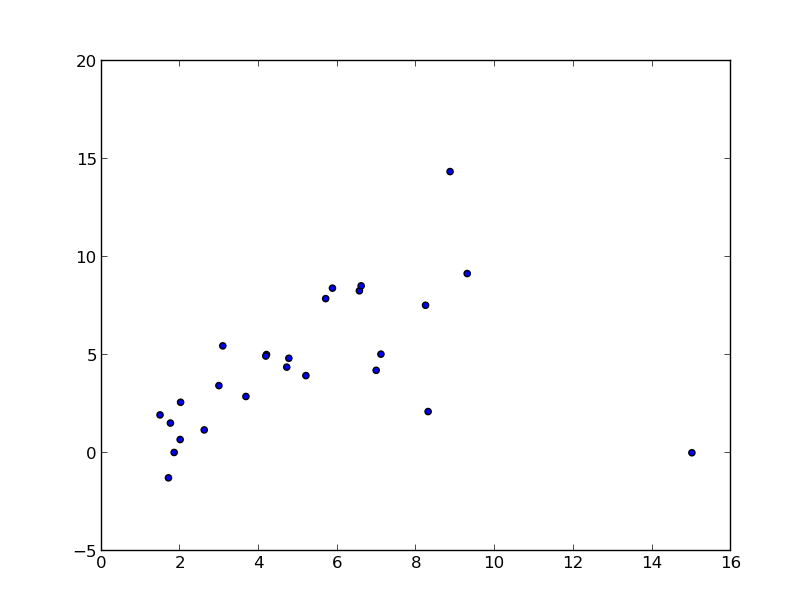
\includegraphics[scale=0.5]{regression.png}
\end{frame}

\begin{frame}
  \frametitle{exercise}
  \begin{itemize}
  \item Solve regression as a QP
  \item Compare results with Minimize: $|\sum_i \mbox{residual}_i|$
  \end{itemize}
\end{frame}

\end{document}
